\subsection{Analytical Jacobian -- BDF \& Radau}

Figure \ref{fig:analytic-bdf-radau} illustrates the impact of supplying an exact analytical Jacobian to the fully implicit BDF and Radau solvers. The evaluation is conducted at a spatial resolution of \(N_x = 1000\) with a strict regularization parameter of \(\varepsilon = 10^{-10}\) and solver tolerance of \(10^{-10}\), sweeping the nonlinearity index \(p\) from 4 to 7. Both solvers operate in sparse mode; the Jacobian callbacks return either a banded array (LSODA/CVODE) or a sparse matrix (BDF/Radau).

For the BDF method, transitioning from an internal finite-difference approximation to an analytical Jacobian reduces execution time by approximately half across the tested indices. At \(p = 6\), the runtime decreases from 17.7 seconds to 7.25 seconds, representing a 2.44\(\times\) speedup. The Radau solver exhibits an even more pronounced improvement: at the same index (\(p = 6\)), the analytical formulation accelerates integration by nearly a factor of four (15.4 seconds compared to 61.2 seconds). Because the internal evaluation metrics (nfev, njev, and nlu) remain nearly identical between the two configurations, the observed performance gains stem exclusively from bypassing the repeated finite-difference evaluations required to construct the numerical Jacobian.

These results indicate that for fully implicit architectures like BDF and Radau from the \pkg{SciPy} suite, explicitly defining the analytical Jacobian yields substantial computational efficiency once the system enters highly nonlinear regimes. The reduction in wall-time firmly justifies the initial implementation effort required to derive the exact derivative, whether calculated manually or via automatic differentiation tools.

\begin{figure}[H]
  \centering
  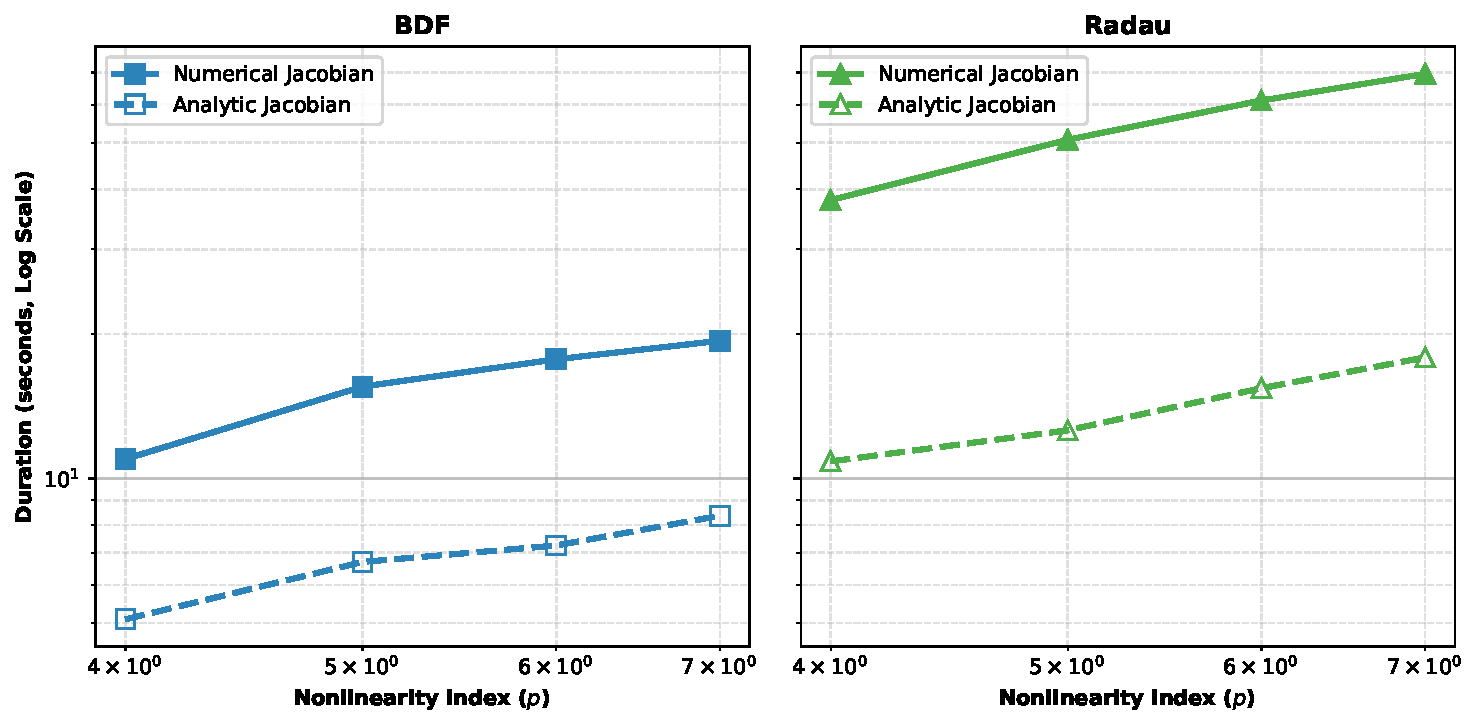
\includegraphics[width=\textwidth]{images/fdm_analytic_comparison_bdf_radau.pdf}
  \caption{Impact of analytical vs.\ numerical Jacobian for BDF and Radau across increasing \(p\) (\(N_x = 1000\), \(\varepsilon = 10^{-10}\), tolerance \(10^{-10}\)).}
  \label{fig:analytic-bdf-radau}
\end{figure}
